\chapter{Measurement Distance}

This chapter is about finding the minimum range length for \ac{OTA}-measurements. Classically \ac{OTA} conformance testing is carried out in the \ac{FF}, in the \ac{mmW} length this hence to some difficulties. To illustrate that there is an example.

\section{Example: Classical OTA measurement distance}

A \ac{UE} operating at $\SI{28}{\giga\hertz}$ is assumed and shall be tested for the American market. Regarding table \ref{tab:legusa} the maximum frequency to test is $f = \SI{100}{\giga\hertz}$. On the one hand \acp{OEM} wont publish where there antennas are and how wide they are, on the other hand \ac{SE} are unintended radiations, so perhaps the radiating element was not meant to be an antenna. So the so called black box approach has to be taken with no pre knowledge of the \ac{DUT}. In worst case configuration it must be assumed that the coherent radiating elements are spread over the howl aperture of the \ac{DUT}. With that assumption a typical smart phone diameter of $D=\SI{15}{\centi\meter}$ is chosen. This leads to a \ac{FF}-distance (refer to equation \ref{eq:ff}) of 

\begin{equation}
r_{\text{FF}} = \frac{2D^2}{\lambda} = \frac{2D^2\cdot f}{c} = \SI{15}{\meter}.
\end{equation}

This brings two major problems, first the dynamic range and second the costly measurement environment. The \ac{FSPL} is regarding to formula \ref{eq:fspl}:

\begin{equation}
L_{\text{FSPL}} = 20\log_{10}\left(\frac{4\pi r_{\text{FF}} \cdot f}{c}\right)\si{\decibel} = \SI{96}{\decibel}
\end{equation}

With $\SI{15}{\decibel}$ gain from the probe antenna and a noise floor at the \ac{DUT} at $\SI{-23}{\decibelm}$ \ac{EIRP} (to have $\SI{10}{\decibel}$ dynamic range) the resulting power at the probe antenna port would be $P_{\text{Probe Port}} = \SI{-23}{\decibelm}-\SI{96}{\decibel}+\SI{15}{\decibel}=\SI{-104}{\decibelm}$. A Noise Figure of the complete measurement equipment will be at least $\SI{20}{\decibel}$. With that the maximum \ac{RBW} would be 

\begin{equation}
\SI{-174}{\decibelm\per\hertz}+\SI{20}{\decibel}-\left(\SI{-104}{\decibelm}\right)=\SI{-50}{\decibel}\ \Rightarrow\ f_{\text{RBW}}=\SI{100}{\kilo\hertz}.
\end{equation}

The required \ac{RBW} is $\SI{1}{\mega\hertz}$, hence to summation of measurement points and lengthy measurements.\\
The cost of \acp{AC} is mainly dependent of the absorber area and the price of the space for the measurement chamber itself. The absorber area is cubically dependent of the range length.

\section{Simulation}

As demonstrated there is the need to find a smaller range length than \ac{FF} distance for ease and efficient measurements. To evaluate the influence of the measurement distance and the probe antenna this simulation was invented and introduced introduced by Benoit Derat and Gerhard Hamberger \cite{mypaper} and is further developed in the framework of this work.

\subsection{Theory}

\begin{figure}[h]
\centering
\def\svgwidth{0.5\textwidth}
\input{Bilder/simPlot.pdf_tex}
\caption{Abstract TRP measurement}
\label{fig:trpmeas}
\end{figure}

For this simulations three spherical surfaces are needed. First the minimal sphere enclosing the \ac{DUT} $S_1$, second the minimal sphere enclosing the probe antenna $S_2$ and third the measurement sphere $\Sigma$ with radius $R$. The origin of the coordinate system is the phase center of the \ac{DUT} ($x$, $y$ and $z$). A sub coordinate system has it's origin in the phase center of the probe and is aligned with it ($u_\phi$, $u_\theta$ and $u_r$). The \ac{EM} emission of the \ac{DUT} is described by the vector fields $E_1$ and $H_1$; the \ac{EM} emission of the probe antenna is analogue to that $E_2$ and $H_2$.\\
The \ac{TRP} is the cumulated active power flowing through a closed surface enclosing the source. So it is the surface integral over the real part of the Poynting-Vektor \cite{mypaper}. Choosing this surface to be the in figure \ref{fig:trpmeas} depicted surface $S_1$ hence to:

\begin{equation}
\text{TRP}=\frac{1}{2}  \oiint_{S_1} \operatorname{Re}\left[E_1	\times H_1^*\right]dS
\end{equation}

Where $dS$ is the vector surface element oriented towards $u_r$. It can be expressed by using the normal vector $n_\text{Sphere}$, pointing radial from the spheres surface and the surface element introduced in equation \ref{eq:trpint}:

\begin{equation}
dS = n_\text{Sphere}\sin\left(\theta\right) d\theta d\phi
\end{equation}

With that all spherical integrals can be solved numerically by the quadratures introduced in section \ref{sec:quadrature}. With the dot product between the integrand and the normal vector $n_\text{Sphere}$ the three dimensional integrand is projected on the normal vector and the total length is summed up.\\
Because a real antenna only measures the electric $E$ or the magnetic $H$ component of a \ac{EM} wave in ether horizontal $u_\phi$ or vertical $u_\theta$ polarisation the probe must be evaluated. The measured power of the probe antenna $P_\text{meas}$ in any solid angle $\Omega$ is derivable by the in \cite{book} introduced equations of power transmission:

\begin{equation}
P_\text{meas}\left(\Omega\right) = \frac{\big|\oiint_{S_2\left(\Omega\right)}\left(E_1\times H_2 - E_2\times H_1\right)dS\big|^2}{8\oiint_{S_2\left(\Omega\right)}\operatorname{Re}\left[E_2\times H_2^*\right]dS}
\end{equation}

$S_2\left(\Omega\right)$  is the surface enclosing the probe at the position given by the solid angle $\Omega$. The radiated vectorfield of the probe antenna must be known; but the radiating power is irrelevant because the measured power is normalized to it. To derive the \ac{TMP} the measured power must be integrated over the surface $\Sigma$ (compare to figure \ref{fig:trpmeas}): \cite{mypaper}

\begin{equation}
\text{TMP}=\oiint_\Sigma P_\text{meas}\left(\Omega\right)d\Omega = \oiint_\Sigma \frac{\big|\oiint_{S_2\left(\Omega\right)}\left(E_1\times H_2 - E_2\times H_1\right)dS\big|^2}{8\oiint_{S_2\left(\Omega\right)}\operatorname{Re}\left[E_2\times H_2^*\right]dS} d\Omega
\label{eq:trpint}
\end{equation}  

\subsection{Implementation}

For the all quadratures a $\SI{5}{\degree}$ \ac{CSSG} was used. There are three main steps for the implementation of this simulation:

\begin{enumerate}
\item The $E$- and $H$-field of the probe antenna is computed via CST Microwave Studio\texttrademark{} by the integral solver at the $\SI{5}{\degree}$ \ac{CSSG}. If the antenna is more complex and thus unsolvable for the integral solver, the time-domain solver is taken and the antennas characteristics are exported as a \ac{NF}-source which than can be simulated by integral solver. With the integral solver it's possible to compute $E$ and $H$ field components at arbitrary points in the surrounding volume.
\item Referring to equation \ref{eq:trpint} a \ac{TMP}-measurement-simulation consists of the outer integral over the measurement sphere $\Sigma$ and the inner integral over the minimum sphere surrounding the probe $S_2$. This means that for every solid angle $\Omega$ the \ac{EM}-field from the \ac{DUT}-antenna on every sphere $S_2$ needs to be computed. The \ac{CSSG} from sphere $S_2$ is always radial aligned, so that the \ac{EM}-field of the probe antenna is valid for every $\Omega$. With $\Delta\phi=\Delta\theta=\SI{5}{\degree}$ this results in
\begin{equation}
N_\text{TMP}=\left(\left(\frac{\SI{180}{\degree}}{\Delta\theta}+1\right)\cdot\frac{\SI{360}{\degree}}{\Delta\phi}\right)^2=2664^2=7,096,896
\end{equation}
measurement points. This is not feasible with the integral solver from CST Microwave Studio\texttrademark{}. Because of that the \ac{NF}-data is fed in to the \ac{FIAFTA}. Occupying the \ac{FIAFTA} the \ac{EM}-field-calculation at every point in the volume is carried out more efficient.\cite{mypaper} \cite{fiafta}
\item The resulting field data is exported to Matlab\texttrademark{}. There the quadrature of the integral from equation \ref{eq:trpint} is solved and the simulated measurement result is gained.
\end{enumerate} 

For different radii $R$ step two and three are iterated. Furthermore the minimum radius is given by the sum of the radii $R$ of $S_1$ and $S_2$.

\subsection{Set up}

For a universal guideline to choose the optimal measurement distance and probe antenna for \ac{TRP}-measurements some sample antennas must be tested.

\begin{figure}[h]
  \centering
  \subfigure[Rendering Picture]{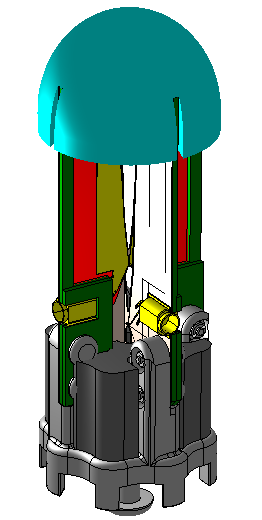
\includegraphics[height=6cm]{Antennas/Vivaldi.png}}
  \centering
  \subfigure[Pattern]{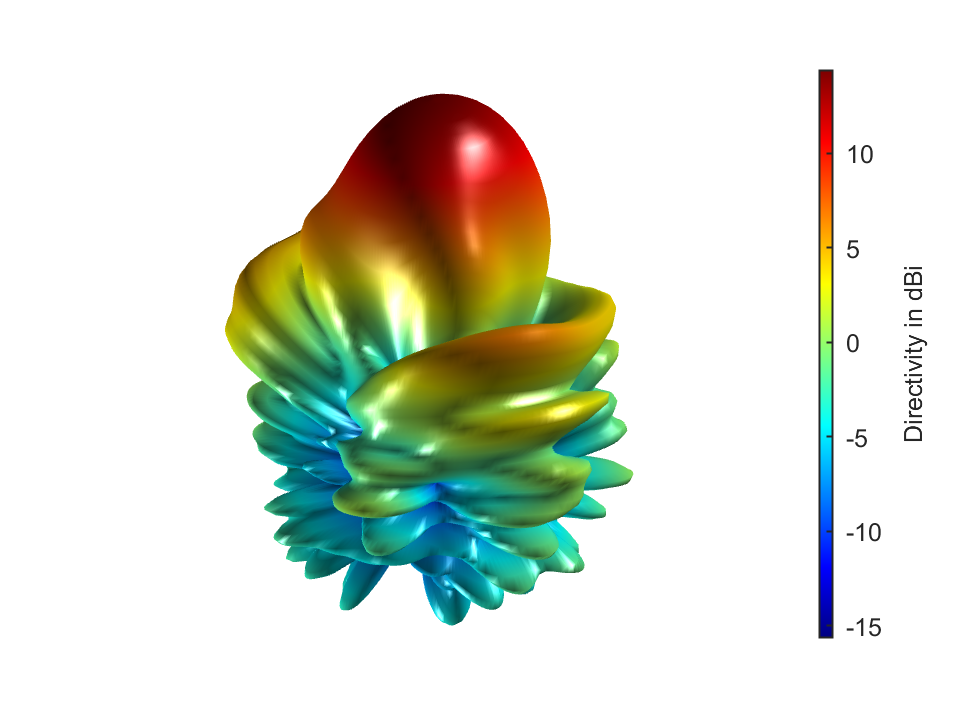
\includegraphics[height=6cm]{Antennas/vivaldi_3D.png}}
\caption{R\&{}S Vivladi TC-TA85CP}
\label{fig:vivpro}
\end{figure}

\begin{figure}[h]
  \centering
  \subfigure[Rendering Picture]{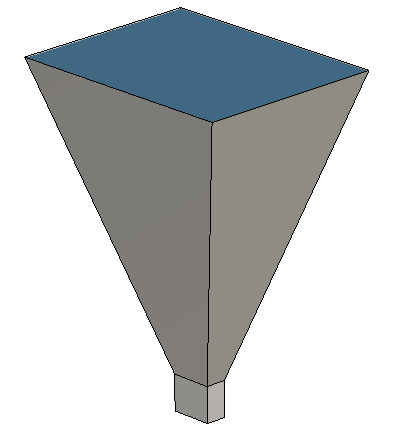
\includegraphics[height=6cm]{Antennas/Horn.png}}
  \centering
  \subfigure[Pattern]{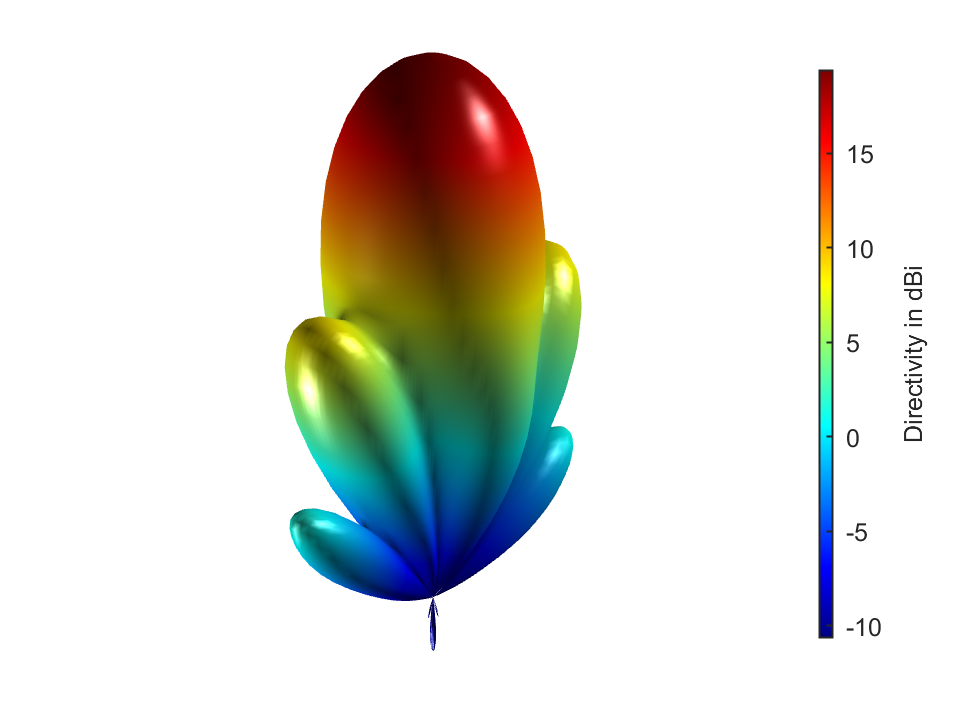
\includegraphics[height=6cm]{Antennas/horn_3D.png}}
\caption{$\SI{20}{\decibel}$ SGH}
\label{fig:hornpro}
\end{figure}

\begin{figure}[h]
  \centering
  \subfigure[Rendering Picture]{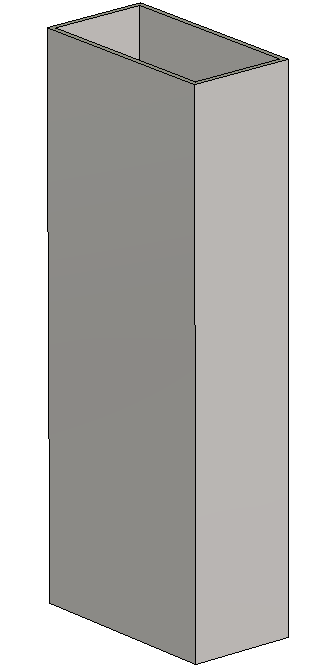
\includegraphics[height=6cm]{Antennas/OEWG.png}}
  \centering
  \subfigure[Pattern]{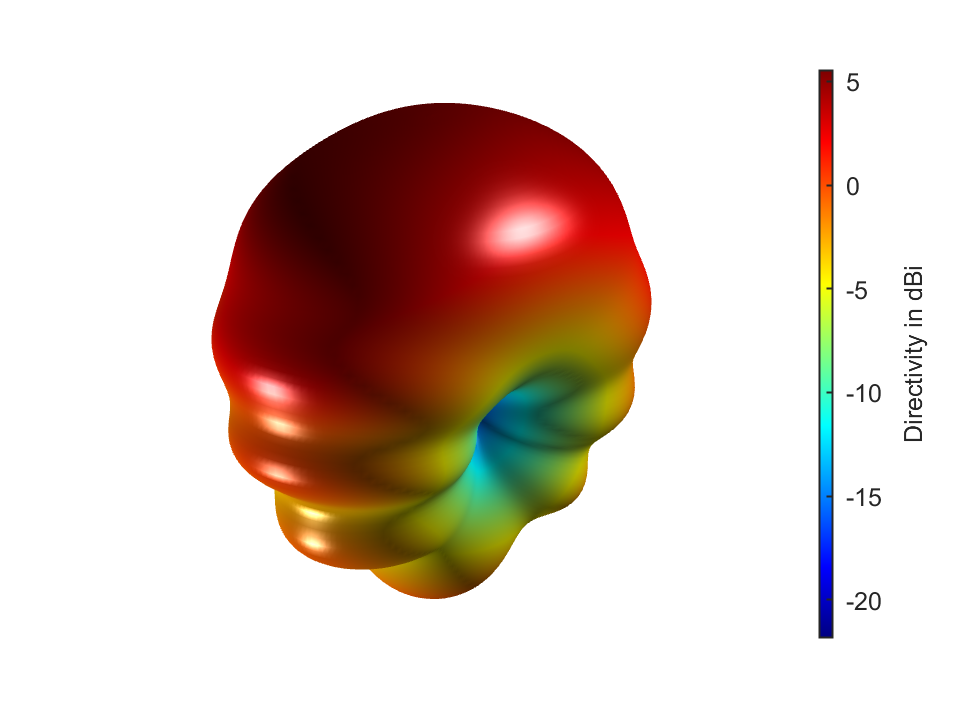
\includegraphics[height=6cm]{Antennas/oewg_3D.png}}
\caption{OEWG}
\label{fig:oewgpro}
\end{figure}


\section{Measurement}